\documentclass[svgnames]{beamer}
\usetheme{Dresden}
\usecolortheme{beaver}
\usepackage{textcomp}
\usepackage{color}
\usepackage{colortbl}
\usepackage{pbox}
\setbeamerfont{page number in head/foot}{size=\large}
\setbeamertemplate{footline}[frame number]
\title{An experimental study of the learnability of congestion control}
\author{Anirudh~Sivaraman, Keith~Winstein, Pratiksha~Thaker, Hari~Balakrishnan}
\institute{MIT CSAIL\vspace{\baselineskip}\\\textcolor{DarkBlue}{http://web.mit.edu/remy/learnability}
}
%\\\textcolor{DarkBlue}{http://web.mit.edu/anirudh/www/sdn-data-plane.html}}
%\date{}
\definecolor{darkgreen}{rgb}{0.0, 0.2, 0.13}

\begin{document}

\begin{frame}

\titlepage

\end{frame}

\begin{Large}
\begin{frame}
\frametitle{Congestion-control protocols today}
\begin{itemize}
\item<2-> Implicit assumptions
\item<3-> Implicit performance goals
\end{itemize}
\end{frame}

\begin{frame}
\frametitle{But, assumptions eventually don't hold}
\begin{itemize}
\item<2-> Links become much faster (transatlantic cables, datacenters)
\item<3-> The number of senders increases (incast)
%\item<3-> Delays get longer: satellite links
\end{itemize}
\end{frame}

\begin{frame}
\frametitle{This talk}
%\begin{itemize}
\begin{center}
\item<1->{How easy is it to “learn” a network protocol to achieve a desired goal,
despite an imperfect set of assumptions?}
\end{center}
%\item<2->{cf. Learning: ``Knowledge acquisition without explicit programming'' (Valiant 1984)}
%\end{itemize}
\end{frame}

\begin{frame}
\frametitle{What we answer}
\begin{itemize}
\item<2-> \textcolor{darkgreen}{Can we tolerate imperfection in link-speed assumptions?}
\item<3-> \textcolor{red}{Can we tolerate imperfection in assumptions regarding the number of senders?}
%\item<3-> \textcolor{darkgreen}{Simplifying topology may be acceptable}
%\item<4-> \textcolor{red}{TCP compatibility is a double-edged sword}
\end{itemize}
\end{frame}

\begin{frame}
\frametitle{Experimental method}
\noindent \only<2>{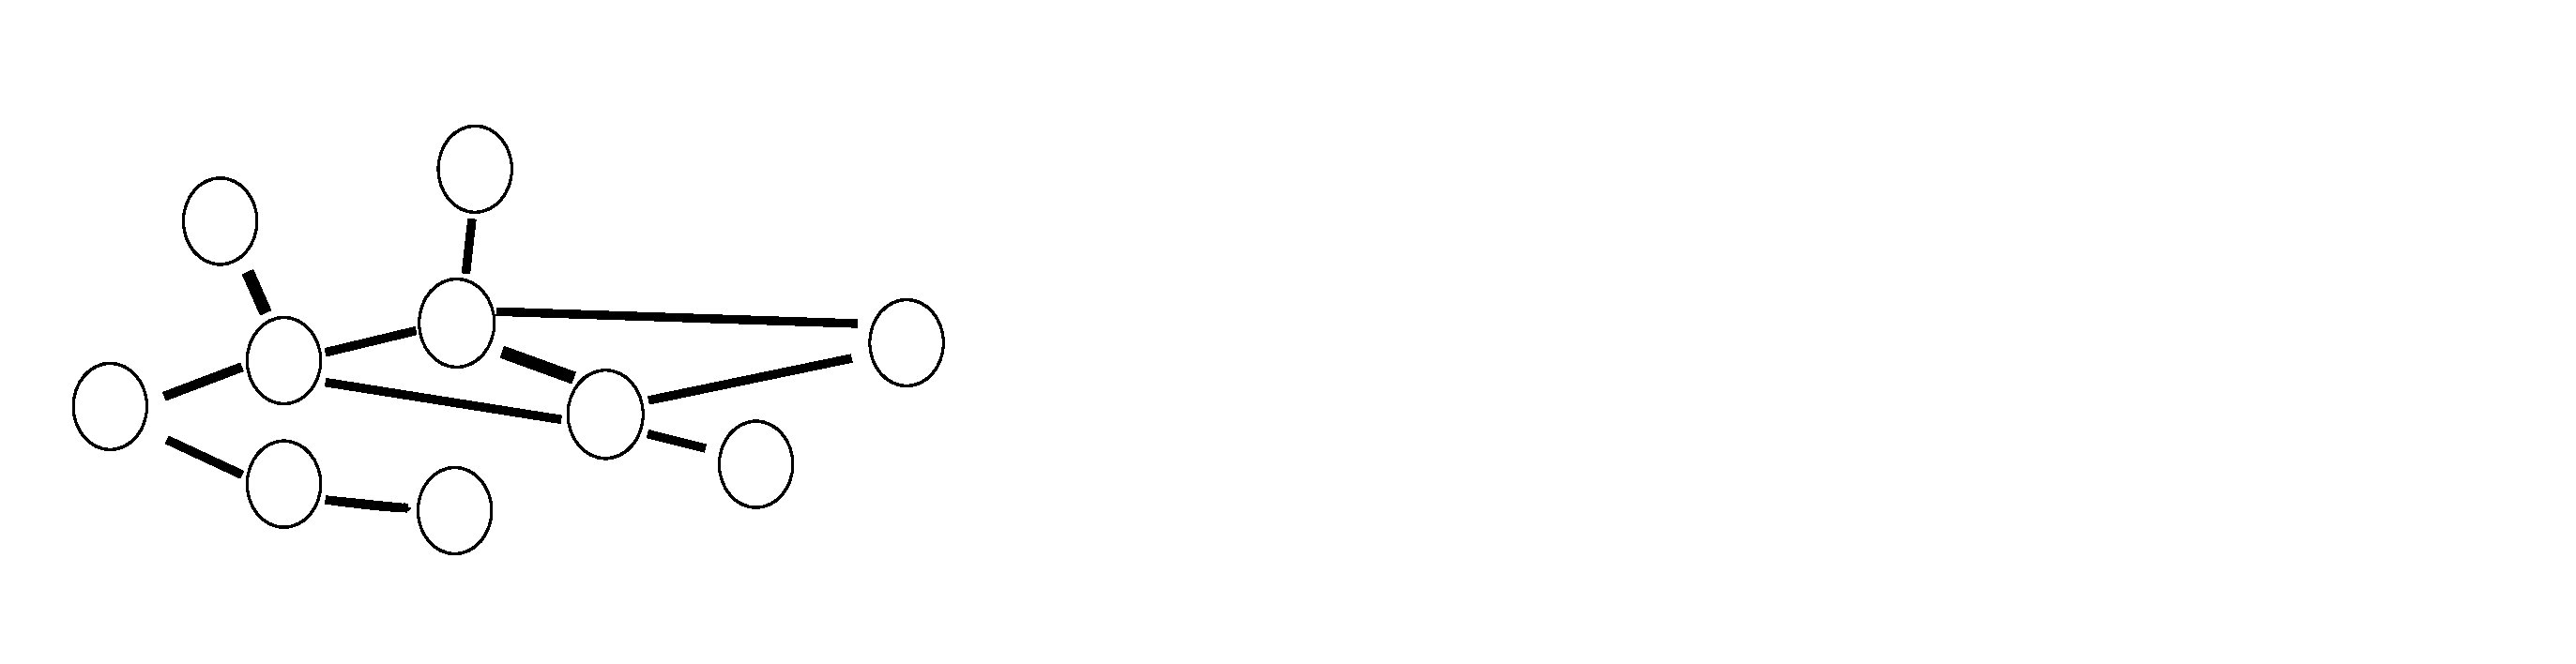
\includegraphics[width=5.5 in]{network-base.pdf}}\only<3>{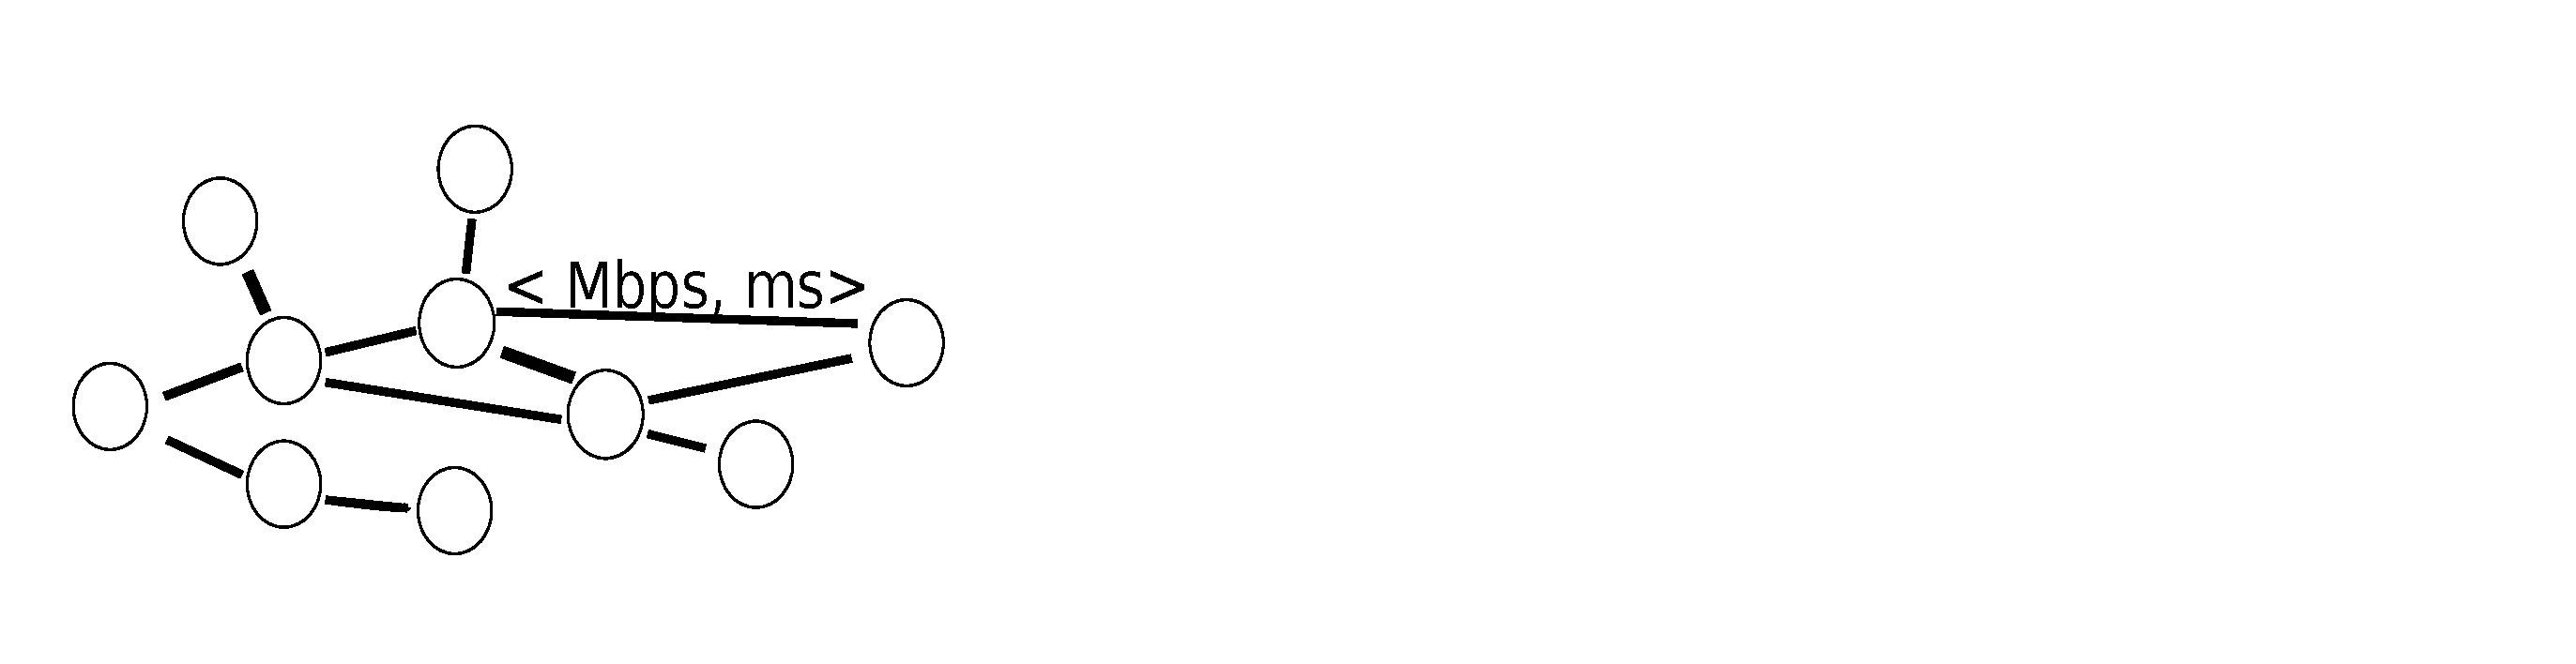
\includegraphics[width=5.5 in]{network-link.pdf}}\only<4>{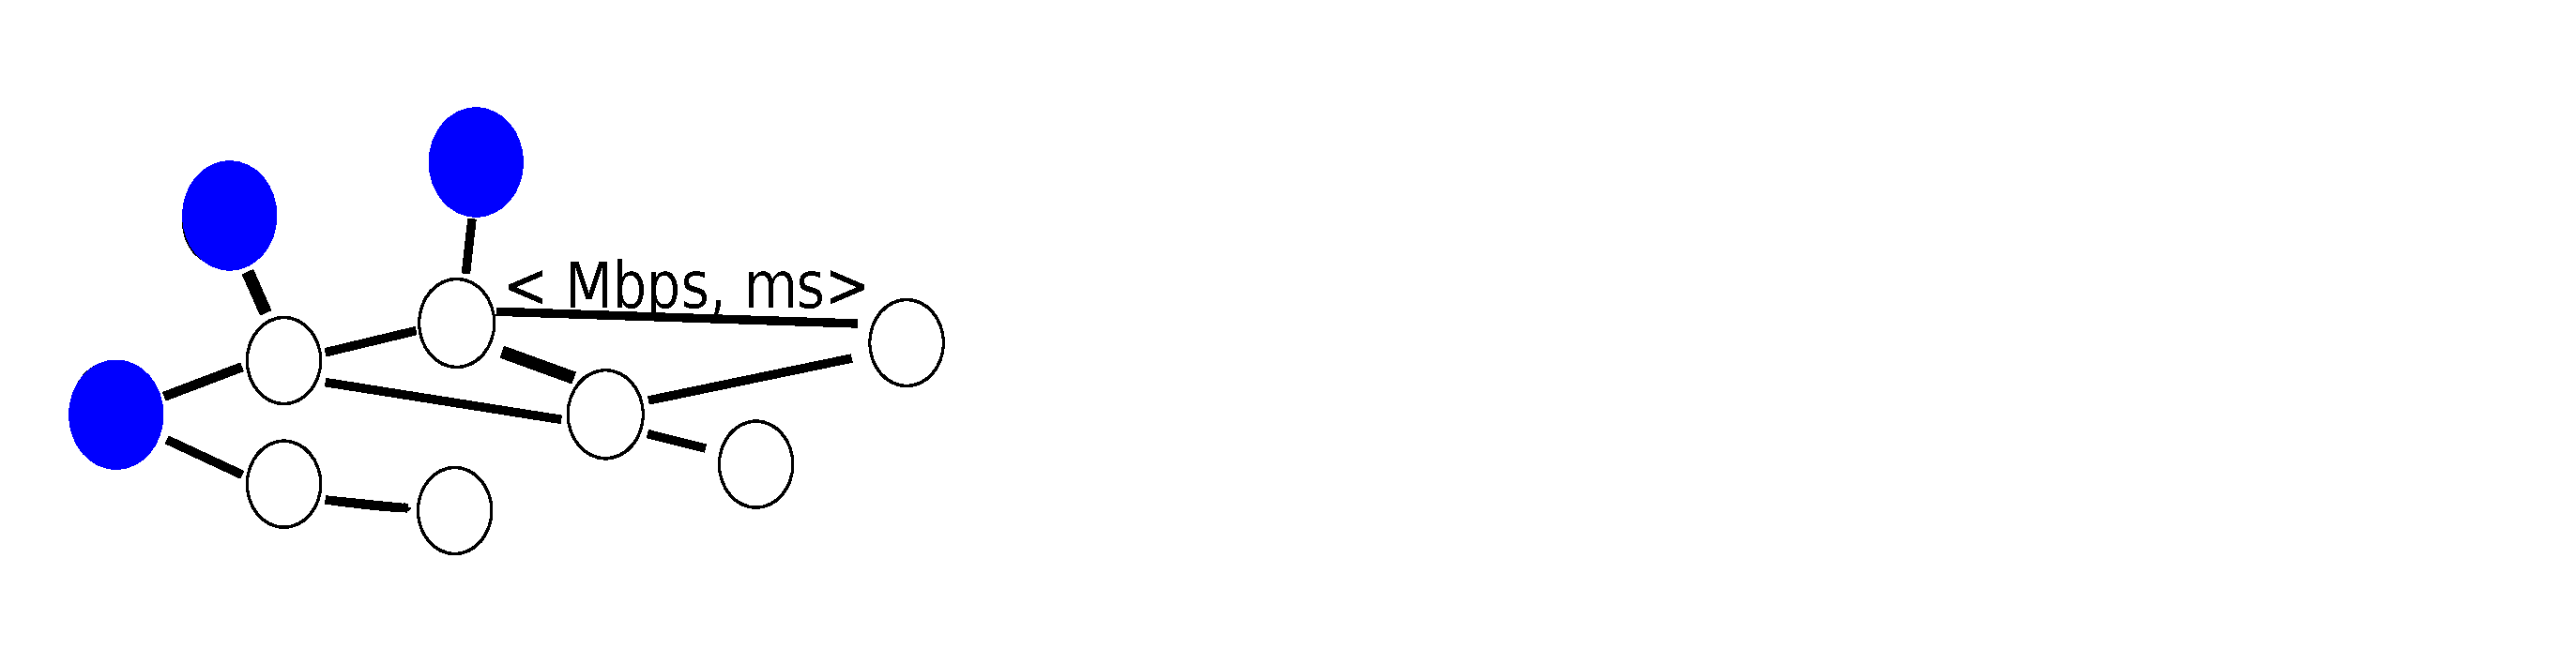
\includegraphics[width=5.5 in]{network-senders.pdf}}\only<5>{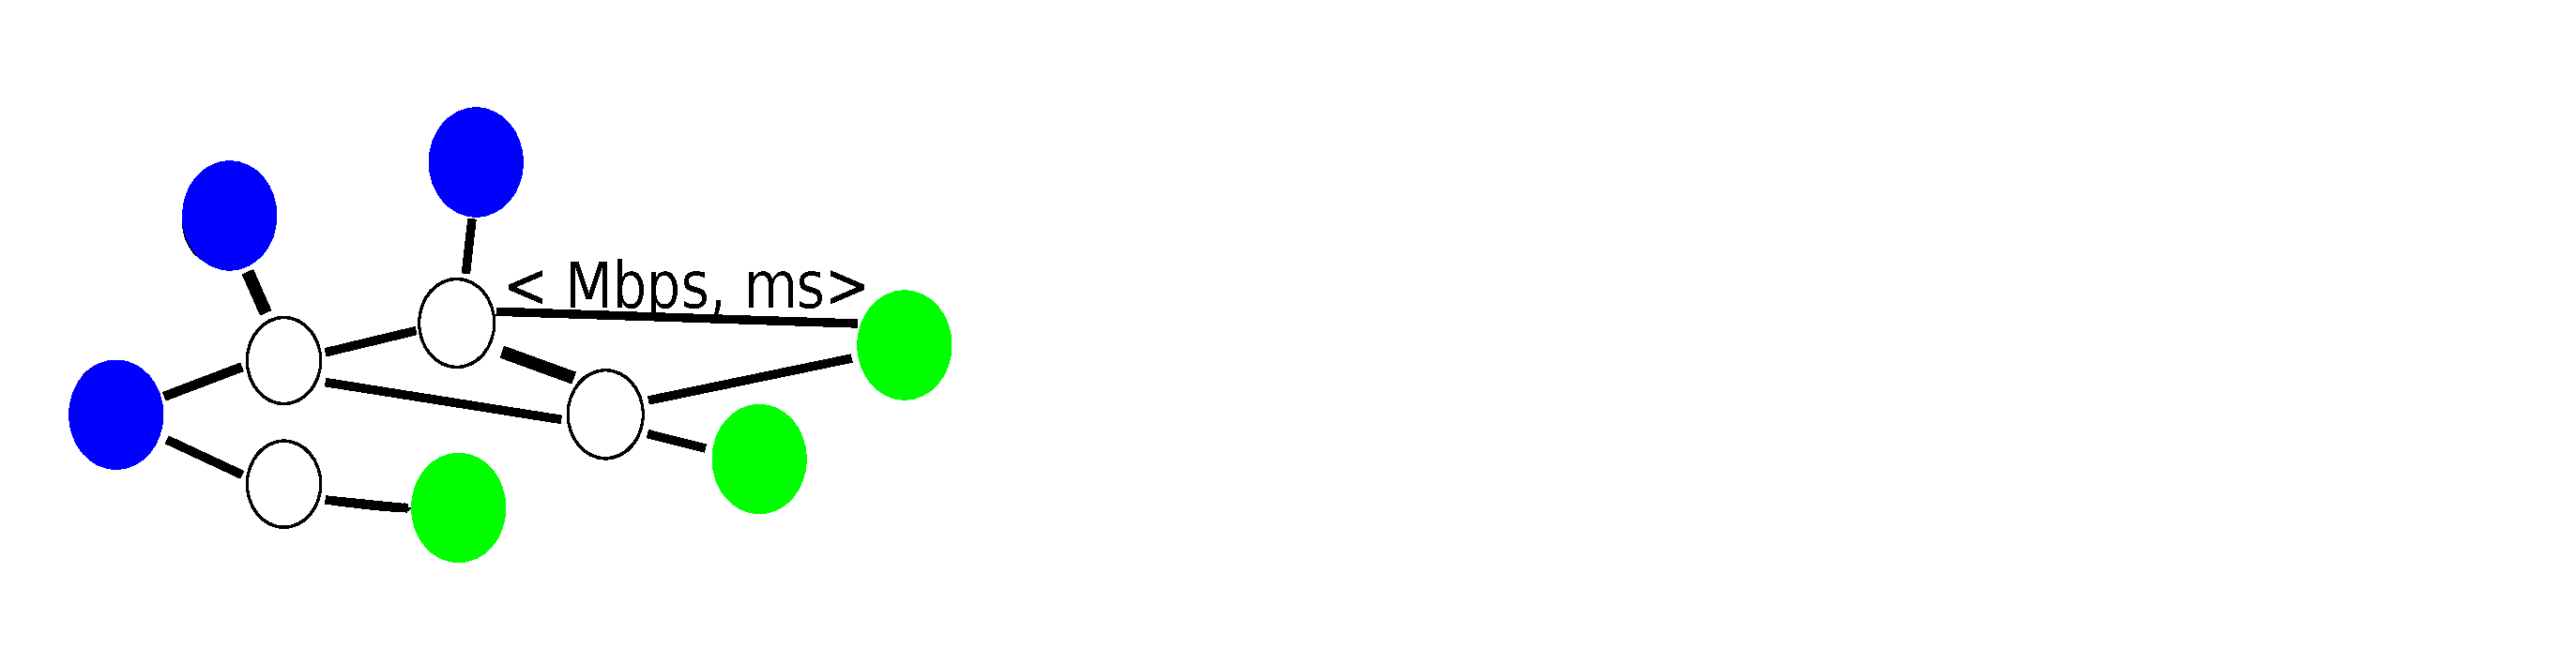
\includegraphics[width=5.5 in]{network-receivers.pdf}}\only<6>{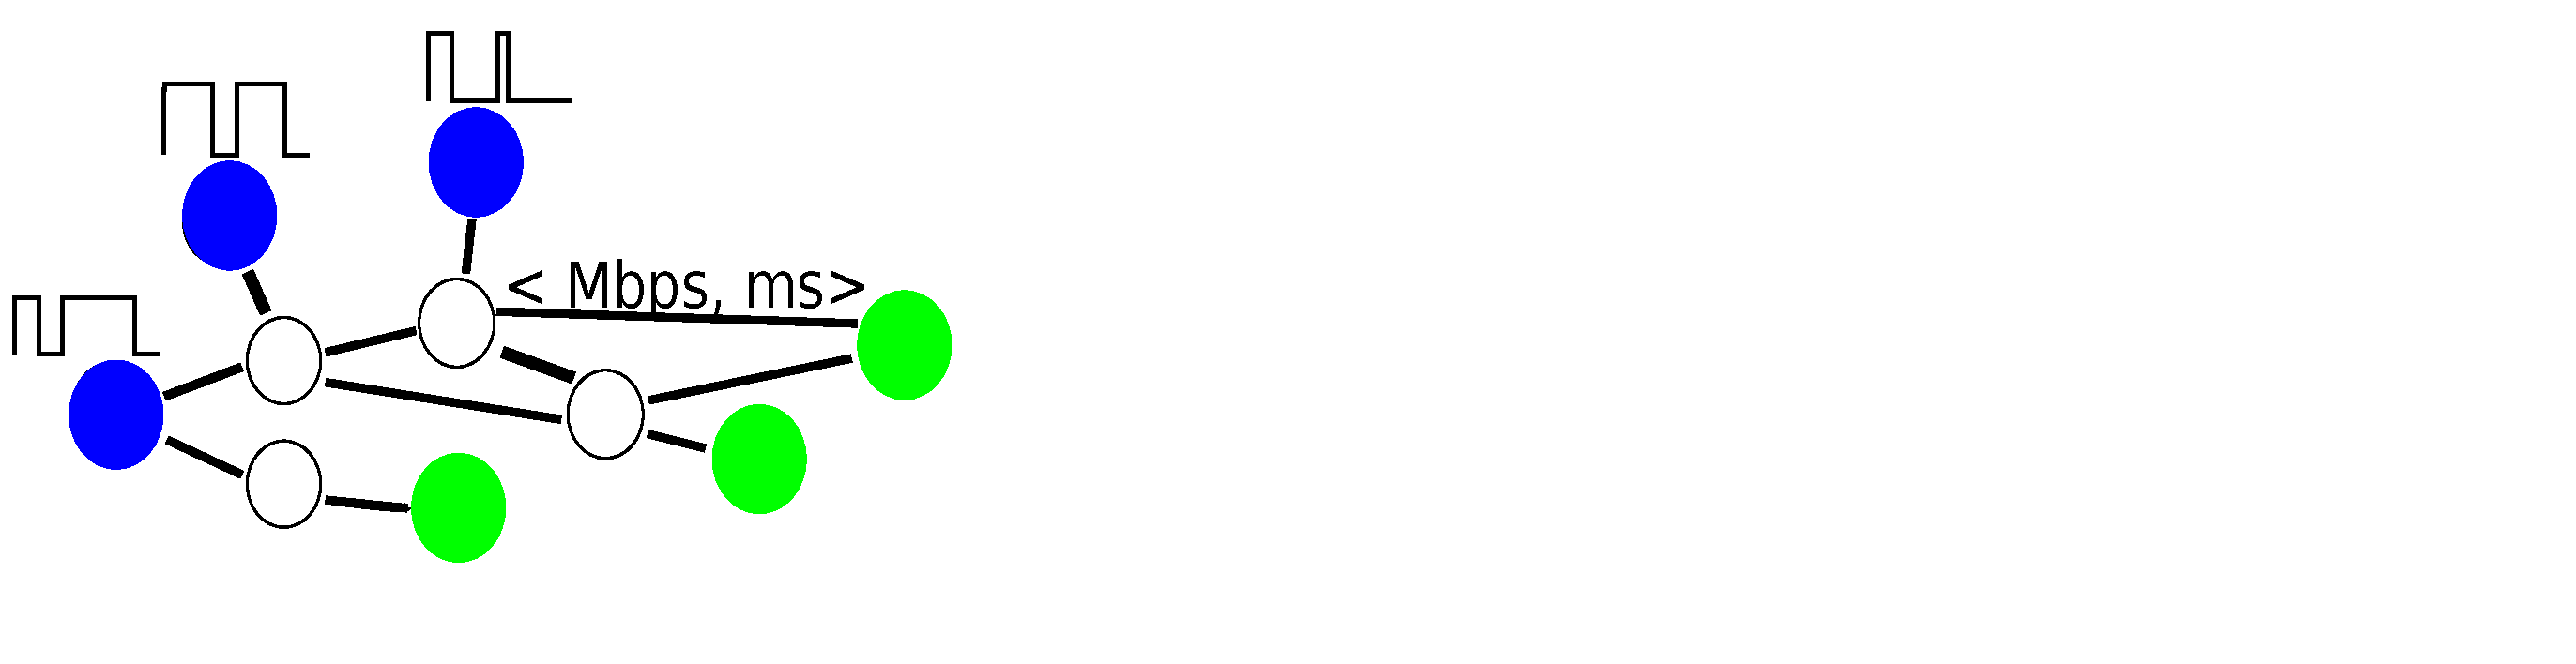
\includegraphics[width=5.5in]{network-application.pdf}}\only<7>{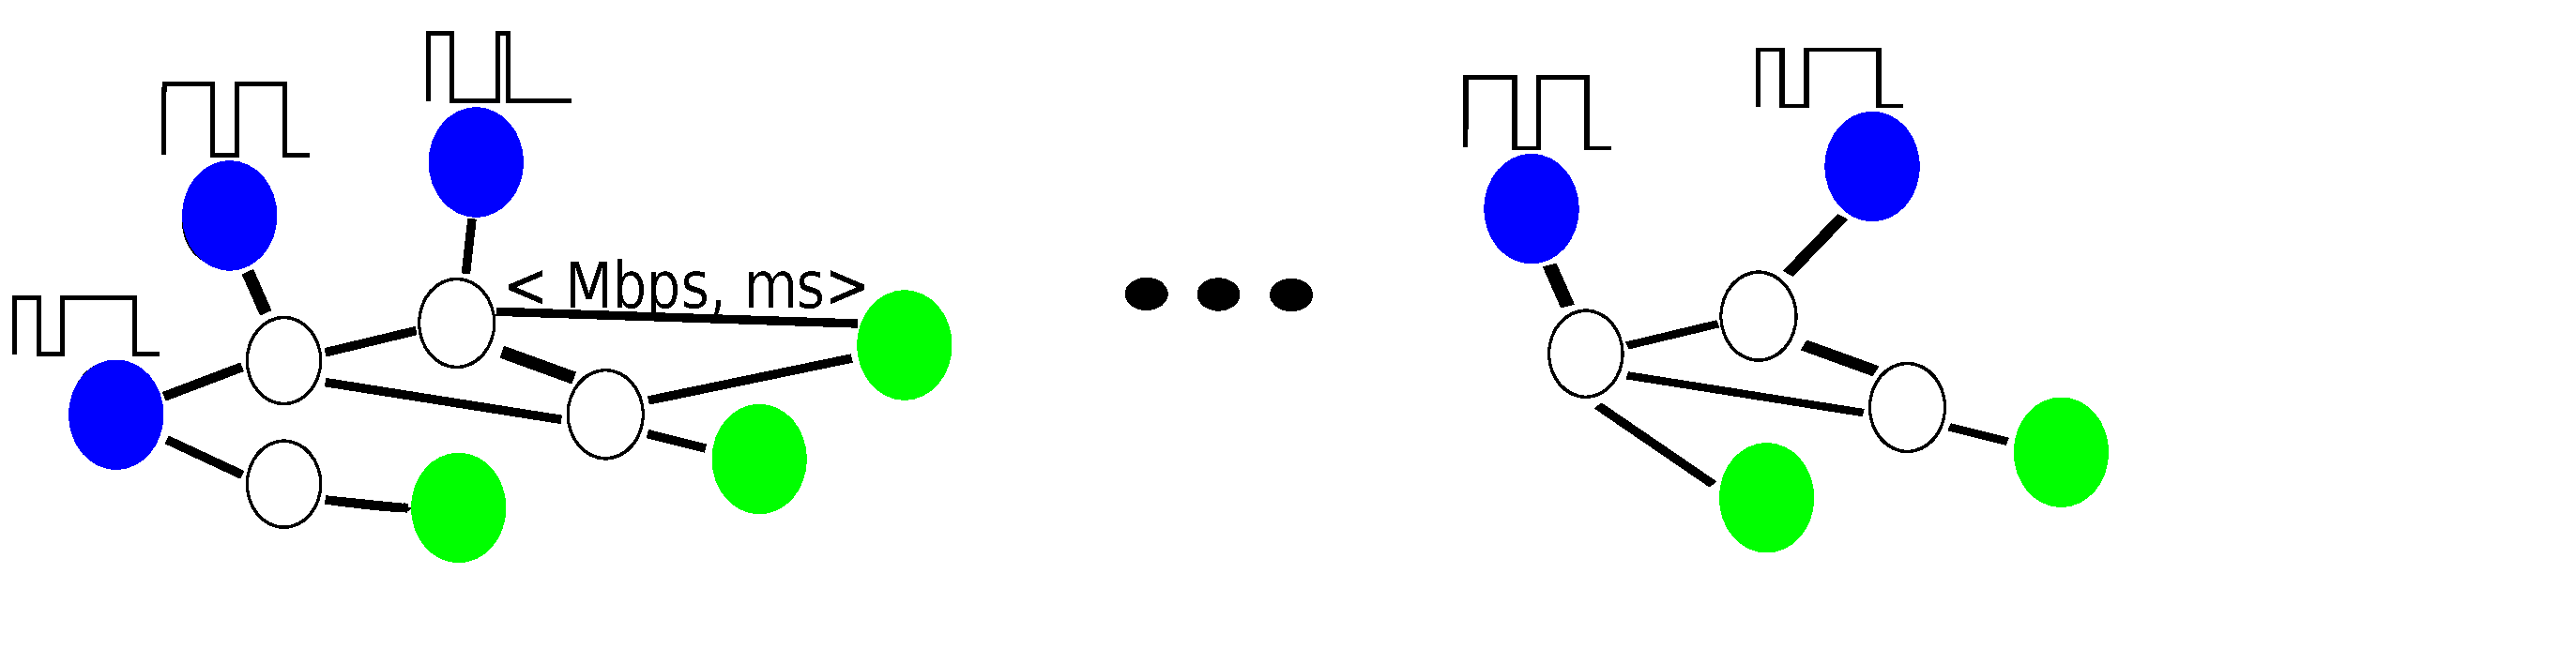
\includegraphics[width=5.5 in]{network-onemore.pdf}}
\end{frame}

\begin{frame}
\frametitle{Experimental method}
\noindent \only<1>{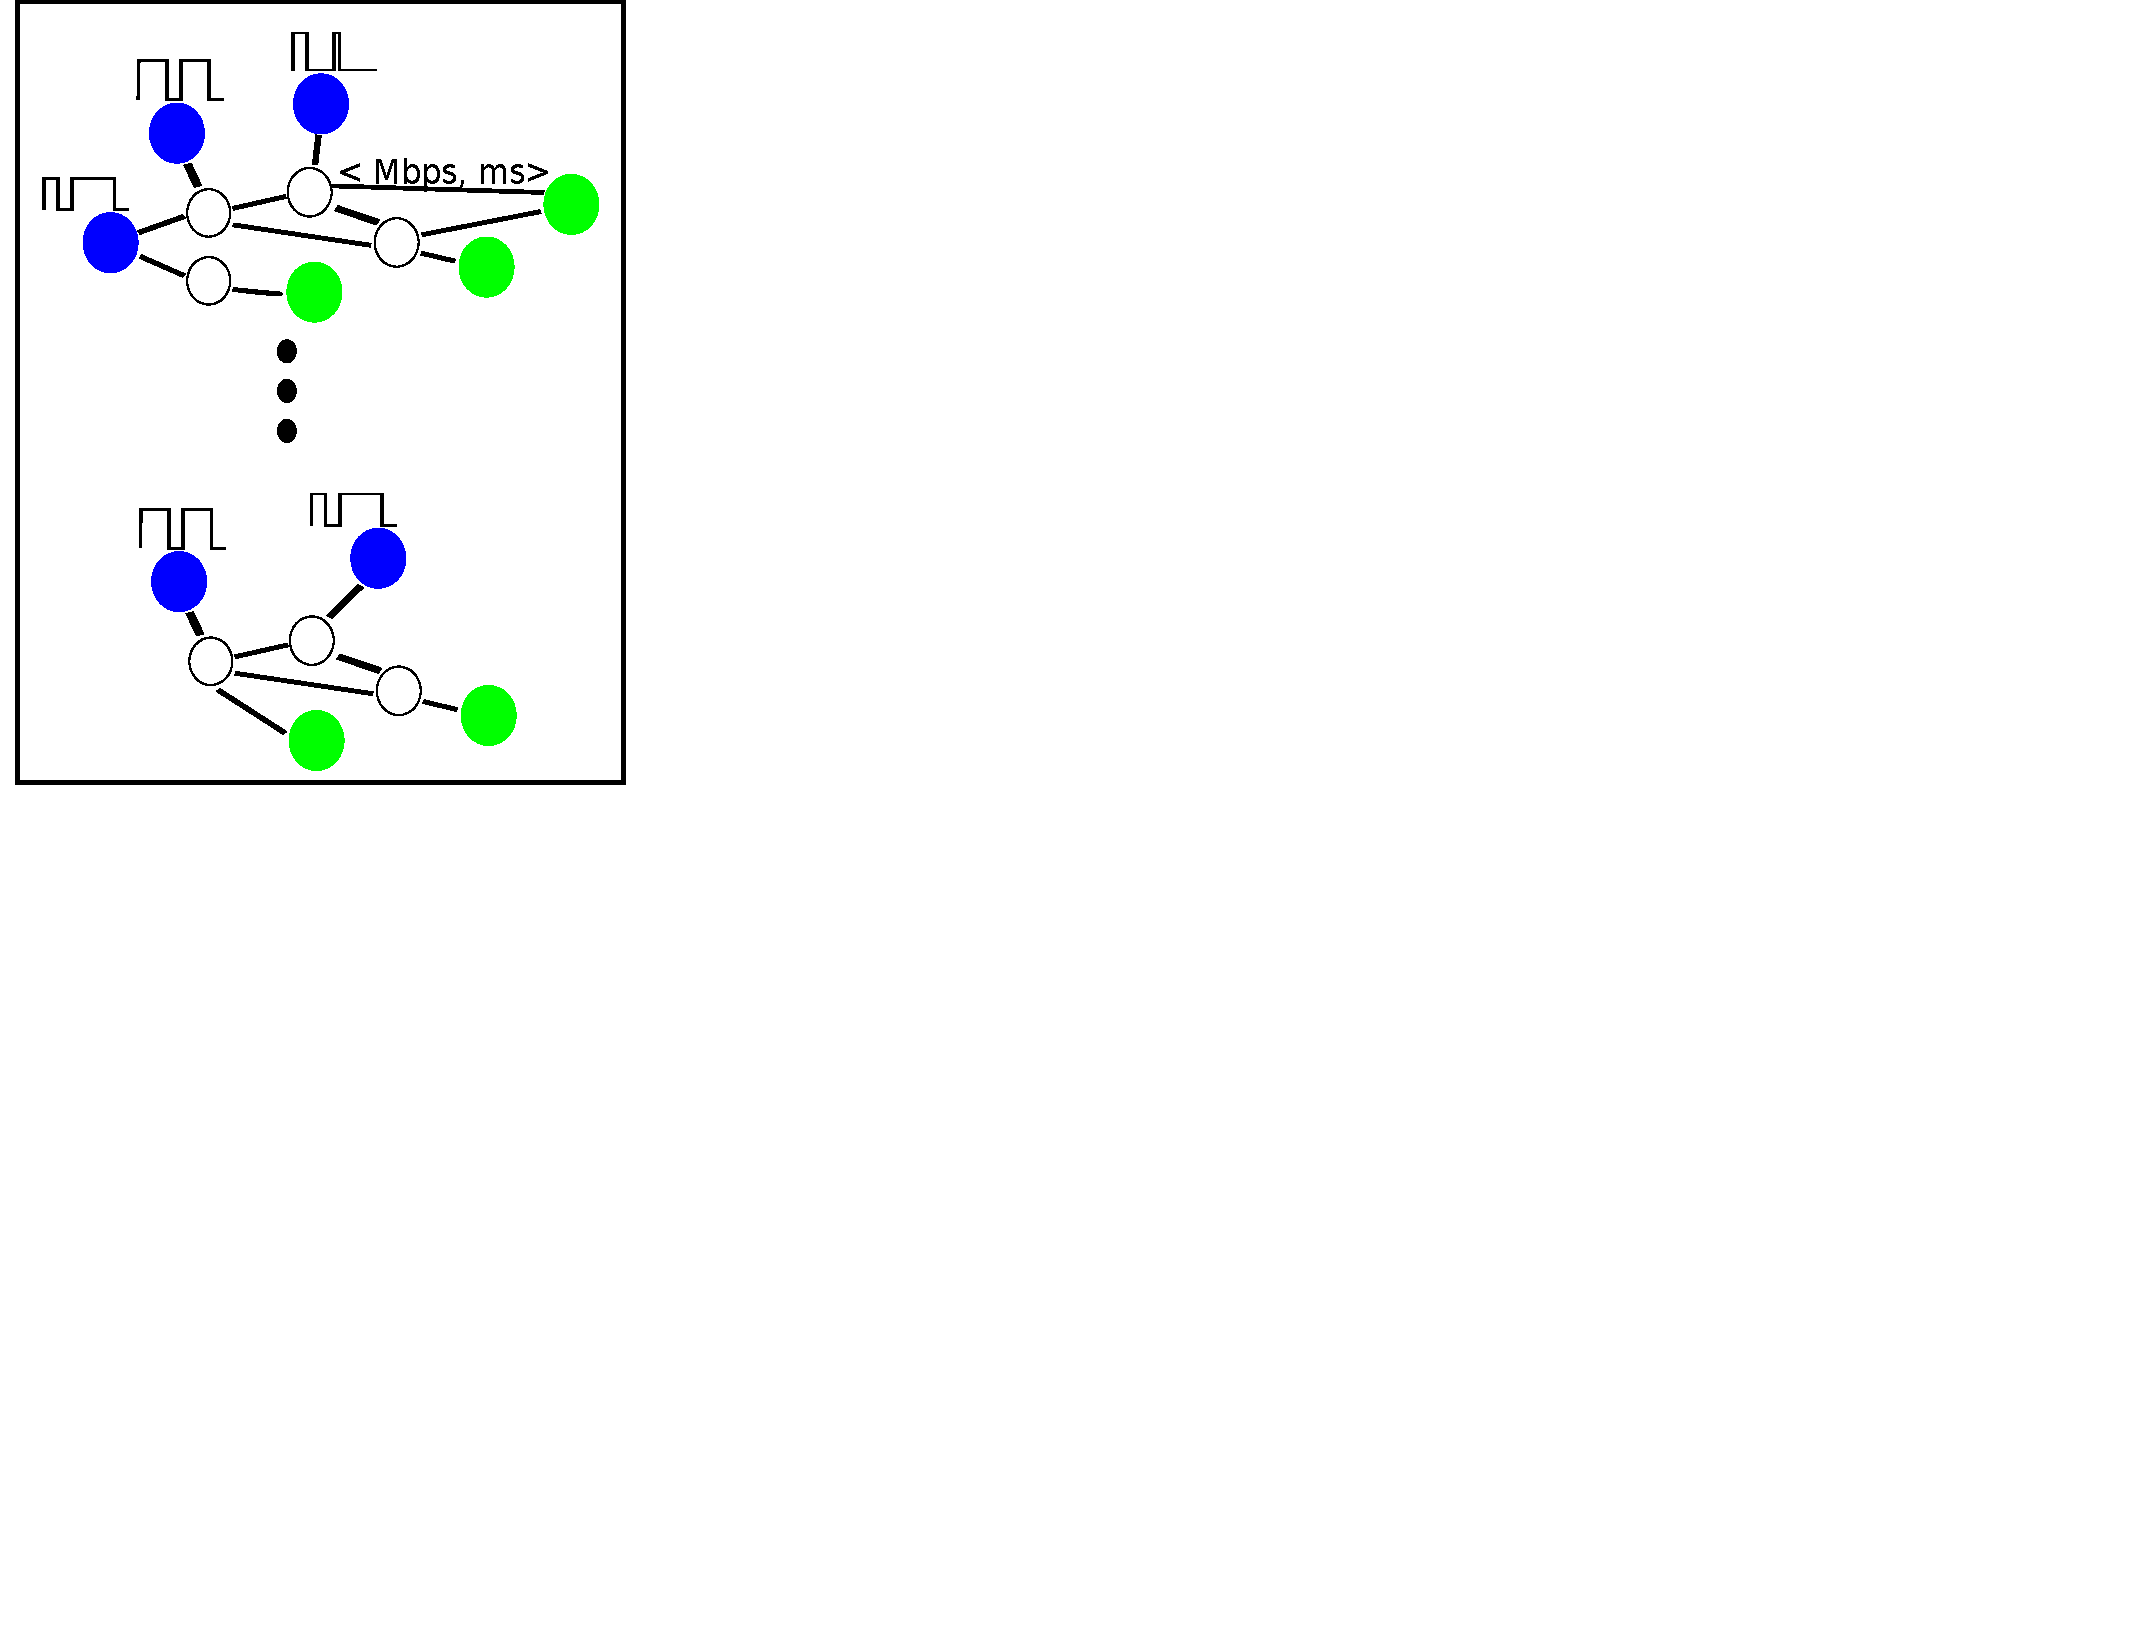
\includegraphics[width=4.5 in]{mechanize-1.pdf}}\only<2>{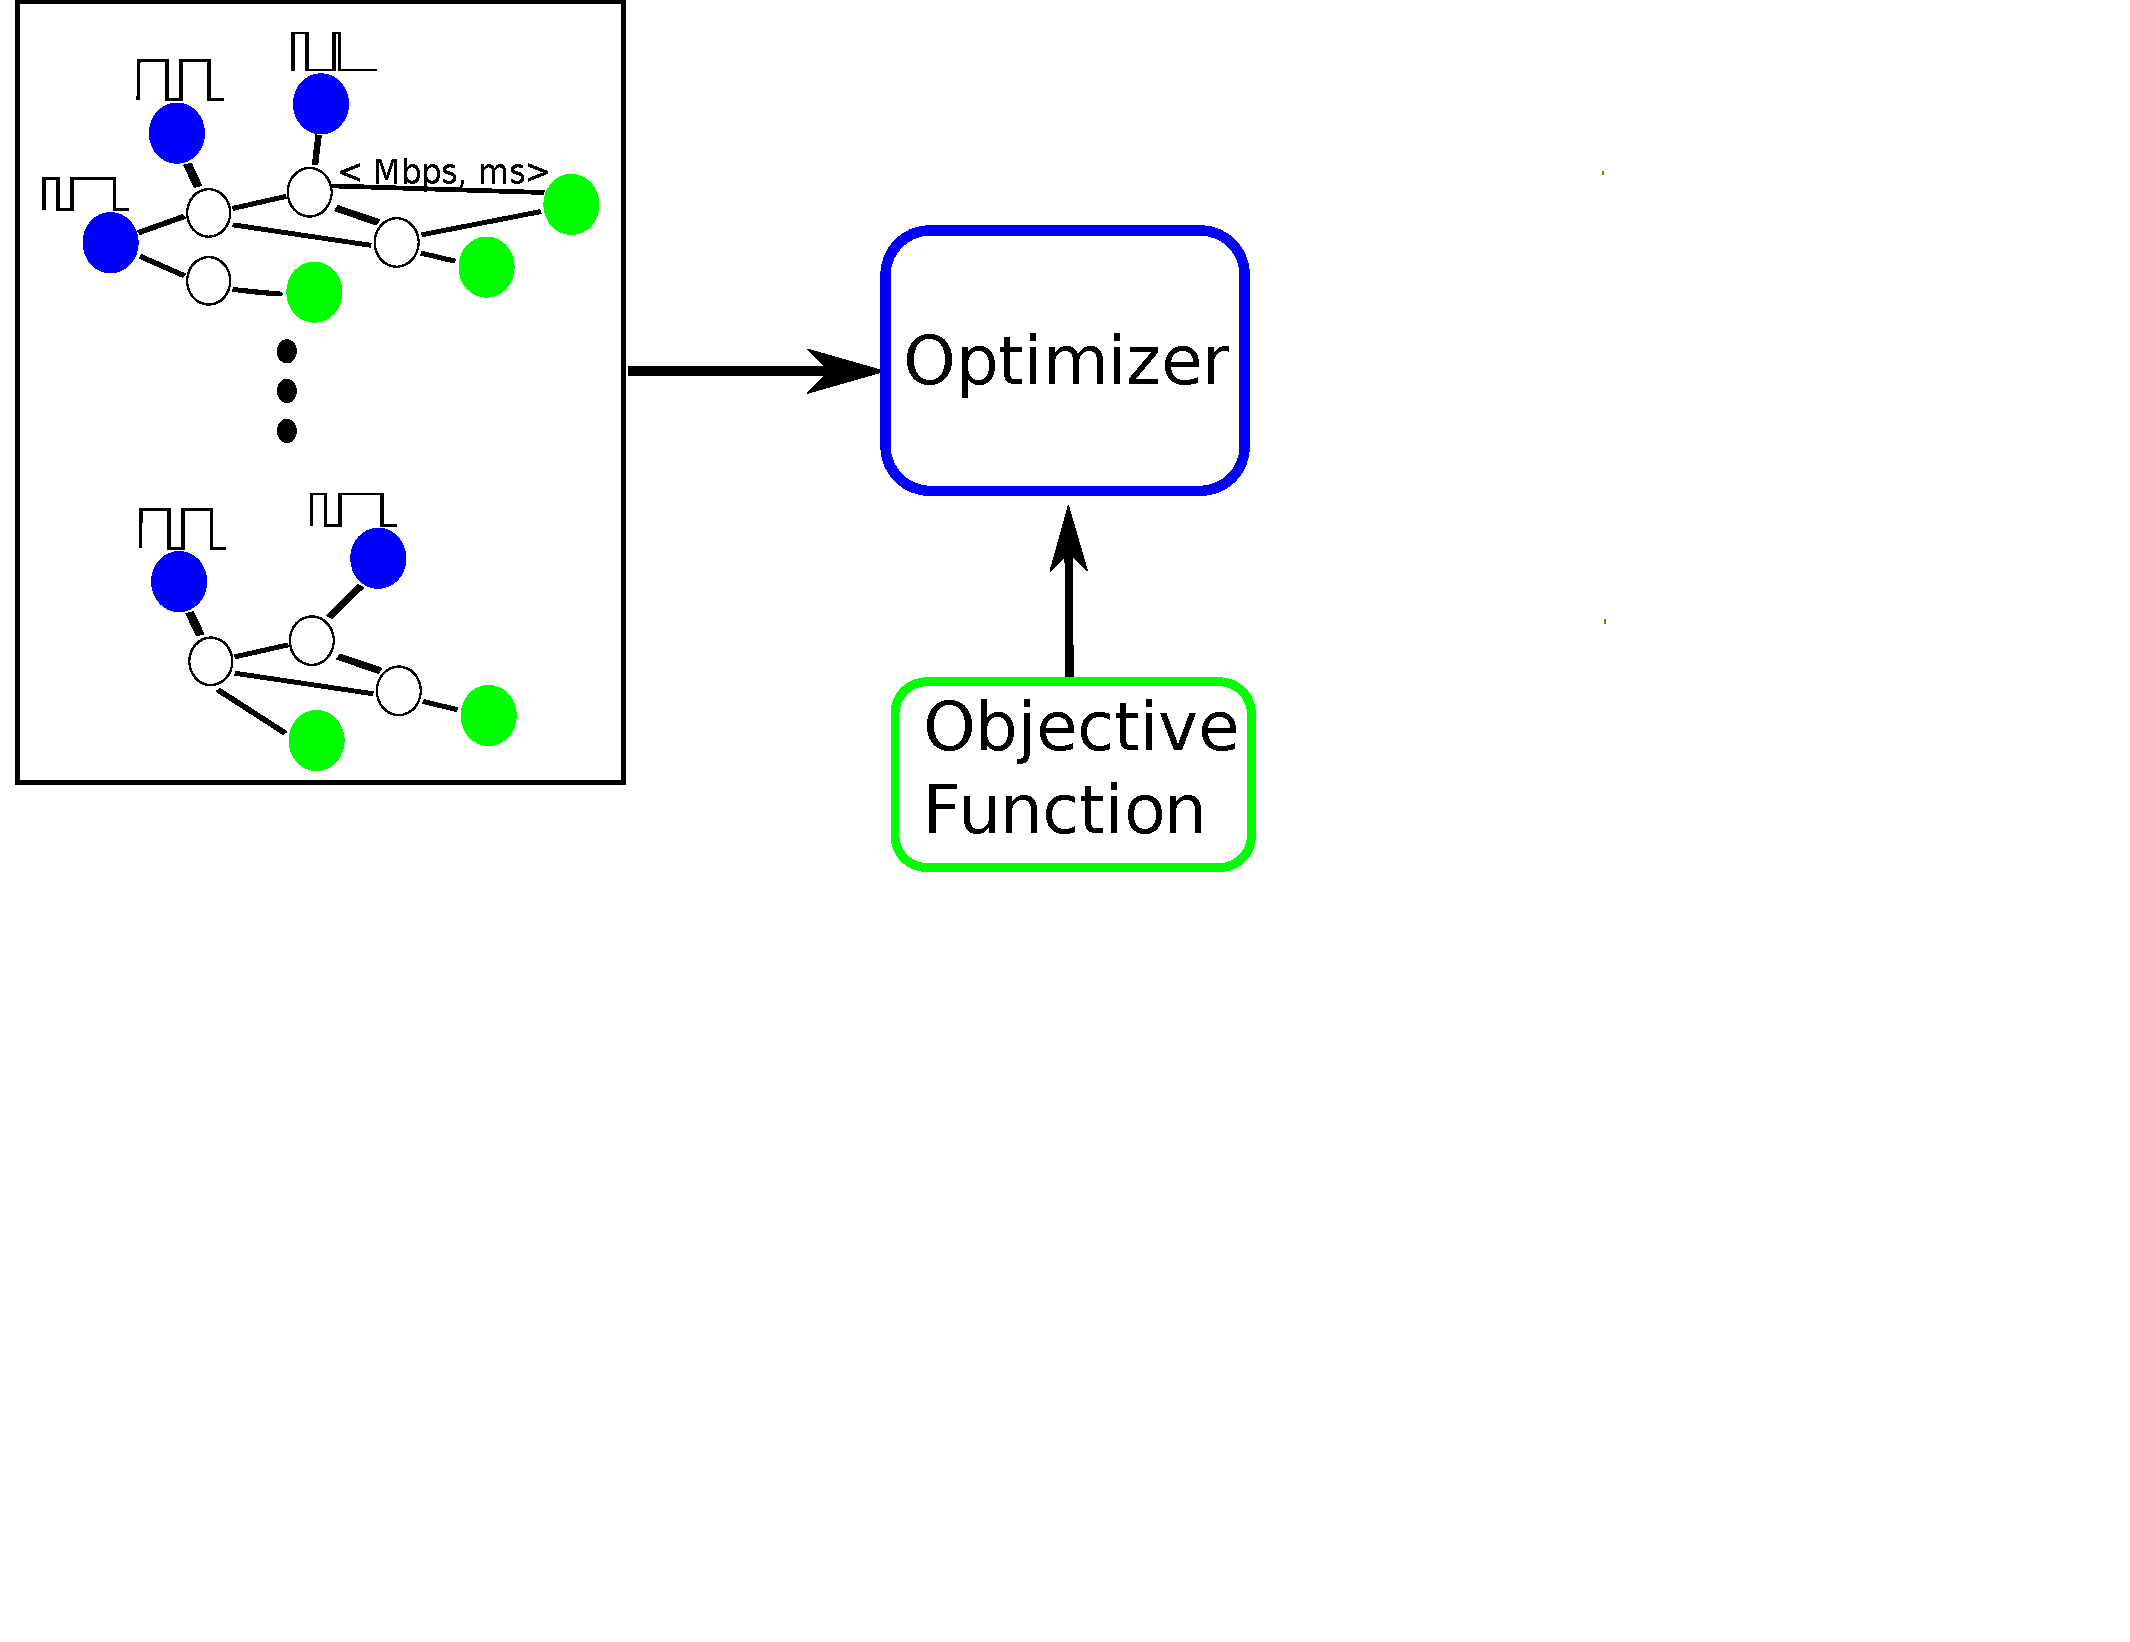
\includegraphics[width=4.5 in]{mechanize-2.pdf}}\only<3>{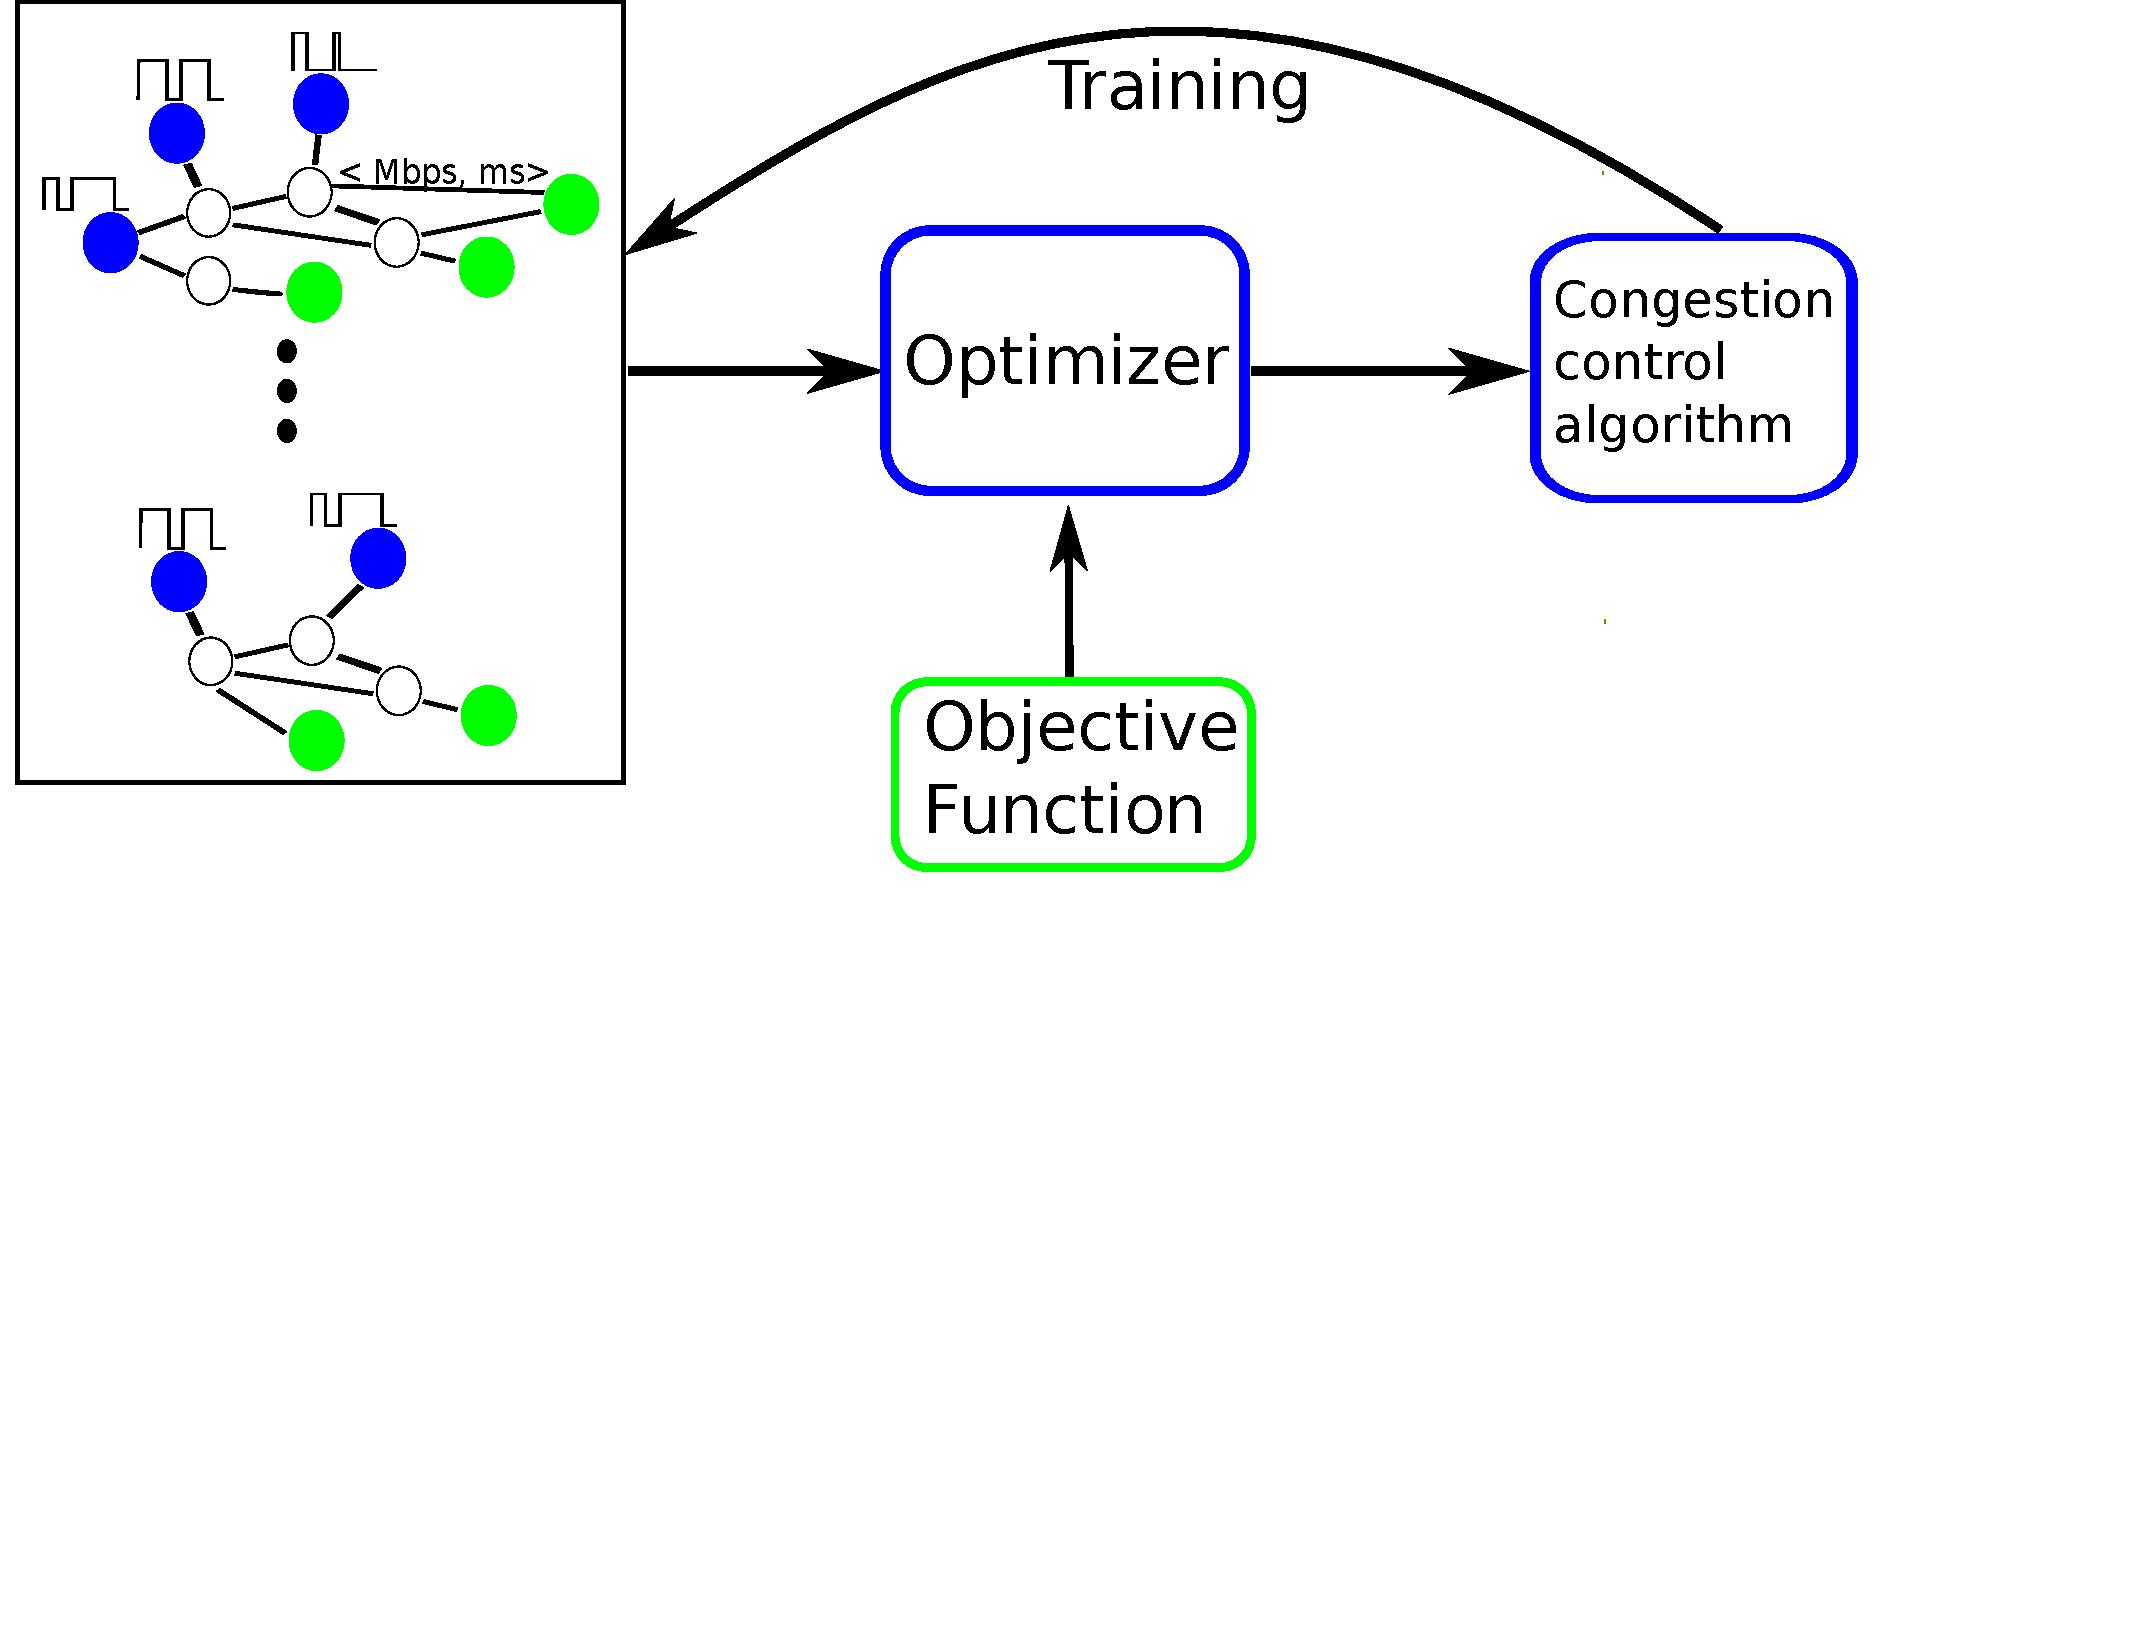
\includegraphics[width=4.5 in]{mechanize-3.pdf}}\only<4>{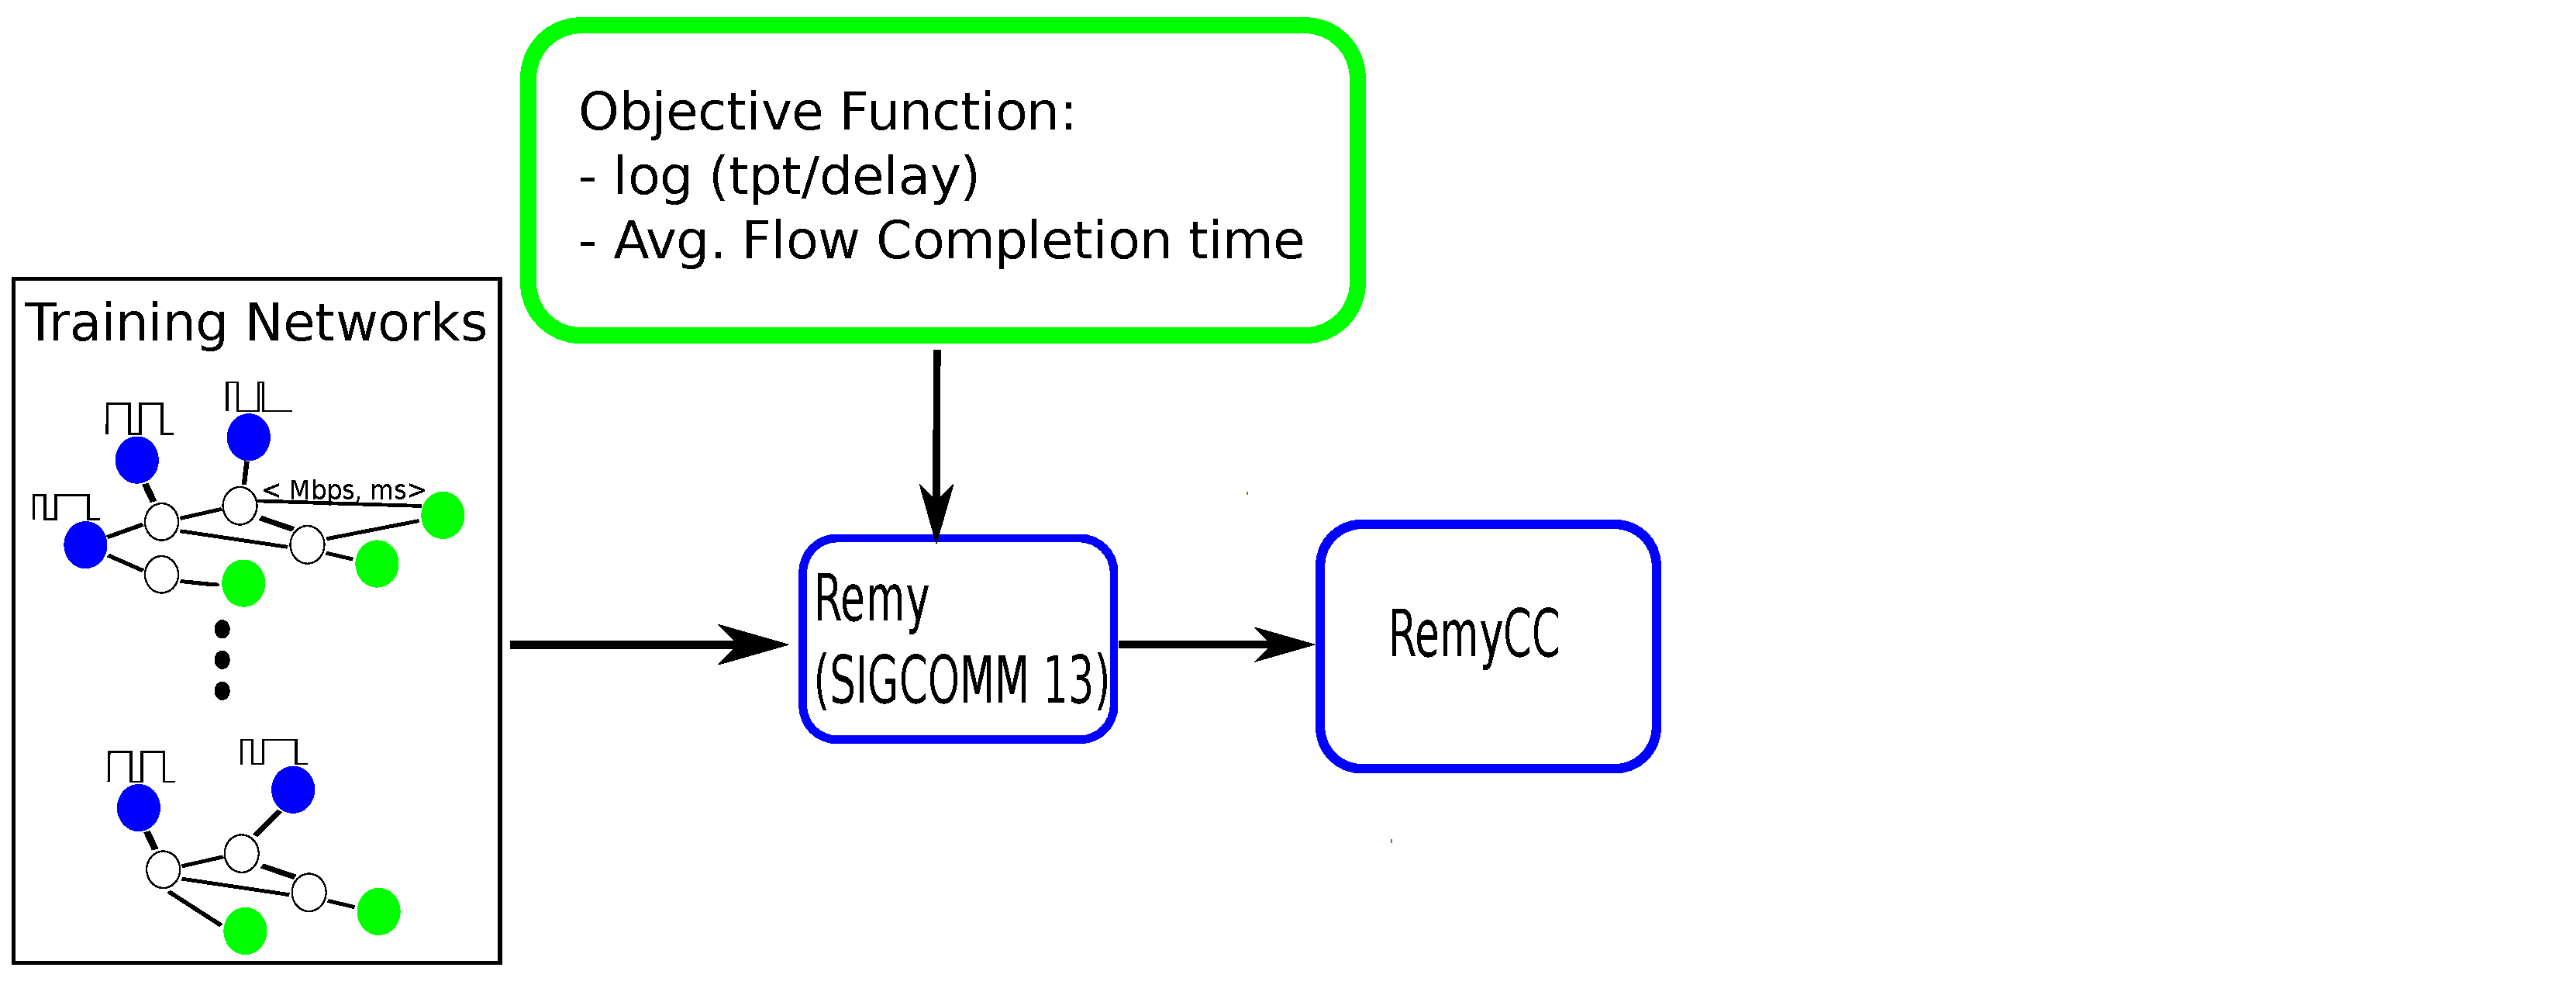
\includegraphics[width=4.5 in]{mechanize-4.pdf}}\only<5>{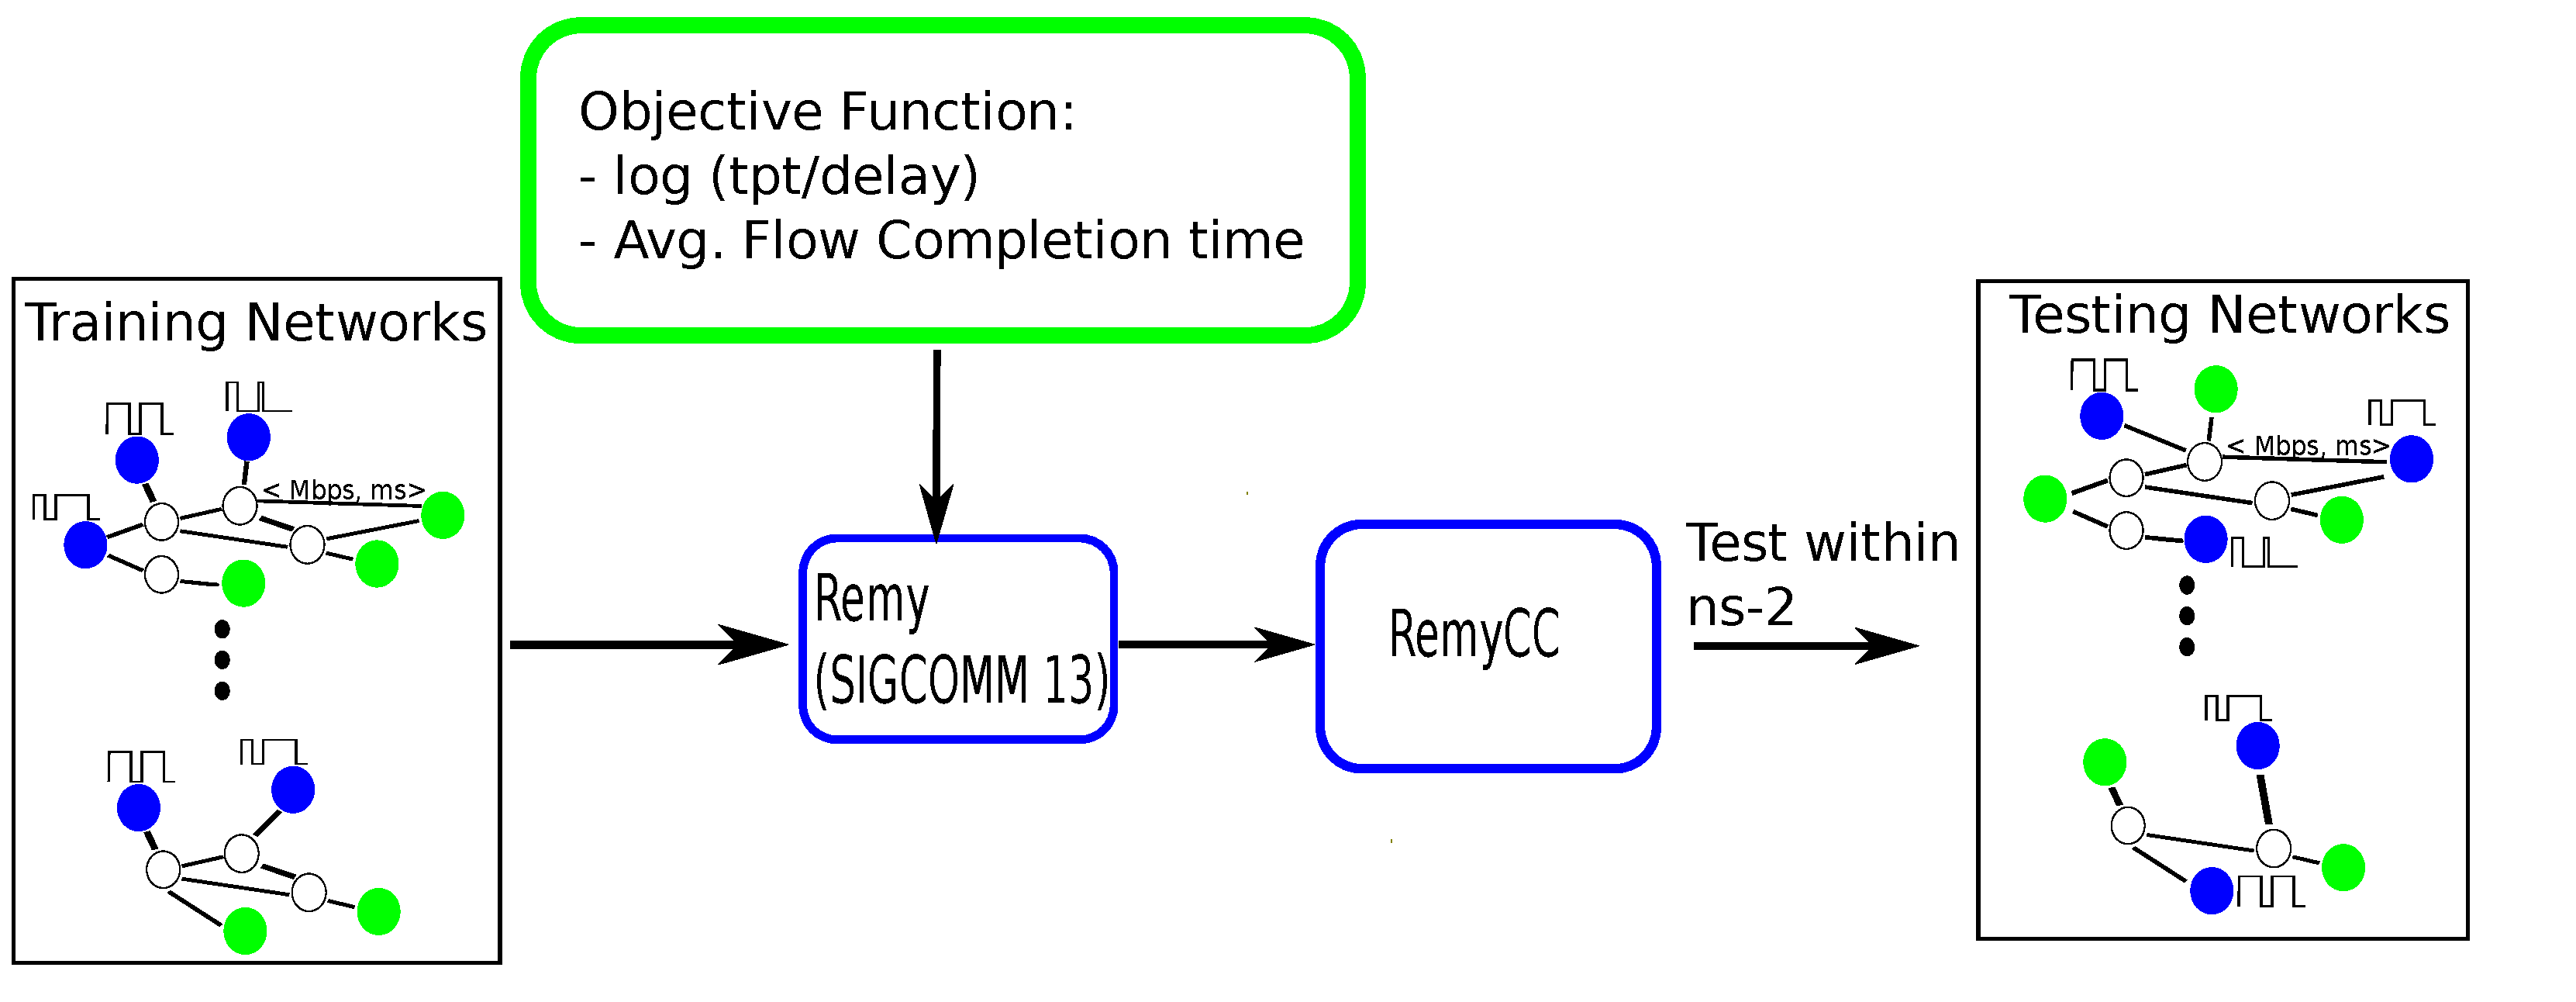
\includegraphics[width=4.5 in]{mechanize-5.pdf}}
\end{frame}

\input optimality

\input linkspeed

\input multiplexing

\input topology 

\input compatibility

\begin{frame}
\frametitle{Limitations}
\begin{itemize}
\item<2-> Remy as a proxy for an optimal protocol design procedure
\item<3-> Results could change with better protocol-synthesis tools
\item<4-> Negative results may no longer hold
\end{itemize}
\end{frame}

\begin{frame}
\frametitle{The learnability of congestion control}
\noindent
\begin{itemize}
\item<2-> \textcolor{darkgreen}{Can tolerate imperfect link-speed assumptions}
\item<3-> \textcolor{red}{Need precision about the number of senders}
\item<4-> \textcolor{darkgreen}{Can tolerate imperfection in the \# of bottlenecks}
\item<5-> \textcolor{red}{TCP compatibility is a double-edged sword}
\item<6-> Ongoing work in using findings to:
\begin{itemize}
\item<2-> improve Google's datacenter transport
\item<3-> user-space implementation of RemyCC
\end{itemize}
\item<7-> http://web.mit.edu/remy/learnability
\end{itemize}
\end{frame}

\end{Large}

\begin{frame}[noframenumbering]
\frametitle{Backup slides}
\end{frame}
\input remy
\input diversity
\end{document}
